\documentclass[twocolumn]{article}
\usepackage{graphicx}
\usepackage{multicol}
\title{EEE3096S Practical 1}
\author{Mutikedzi Mudzanani, Lutendo Mulaisi}

\begin{document}
\maketitle

\section{Introduction}
Run-time speed of a program on a computer depends on many parameters. Some of the parameters are threads, compiler-flag and the width of the bits the program is using. Research shows that the number of threads are not exactly proportional to the speed of the program. Compiler flags influences the instructions to be executed. The bit-width are the slots of memory that the values in the program are stored in.
\section{Method}
\subsection{Running different threads}
This experiment consist running a program with 2, 4, 8, 16 and 32 threads. The program is ran five times and the average of the times are taken. The thread count with the smallest average is then taken to run with different flags.
\subsection{Running different flags}
Just like running different threads, the different flags are compiled and ran for five times then the average is taken. Again, the flag with the smallest time is taken to run at different bit-width.
\subsection{Running different bit-width}
Finally, the program is ran using different bit-width, five times then get the average. The width with smallest average time is then taken.To determine the best combination, from the above, the best thread count is comined with the best flag count and the best width count.

\section{Results}
\begin{table}[!ht]
    \centering
    \caption{Running different flags with 4 threads}
    \begin{tabular}{|l|l|}
    \hline
        threads & Average time [ms] \\ \hline
        2 & 37,68954 \\ \hline
        4 & 14,6458 \\ \hline
        8 & 27,1508 \\ \hline
        16 & 23,7954 \\ \hline
        32 & 29,5234 \\ \hline
    \end{tabular}
    \label{Table 1}
\end{table}

\begin{table}[!ht]
    \centering
    \caption{Running different flags with 4 threads}
    \begin{tabular}{|l|l|}
    \hline
        Flags & Average time \\ \hline
        O0 & 7,6308 \\ \hline
        O1 & 13,608356 \\ \hline
        O2 & 32,651 \\ \hline
        O3 & 21,6398 \\ \hline
        Ofast & 17,1598 \\ \hline
        Os & 4,18 \\ \hline
        Og & 20,925 \\ \hline
        funroll-loops & 19,8252 \\ \hline
    \end{tabular}
    \label{Table 2}
\end{table}

\begin{table}[!ht]
    \centering
    \caption{Running different bit-width with 4 threads and flag -Os}
    \begin{tabular}{|l|l|}
    \hline
        Data type & Average time \\ \hline
        float (32 bit) & 4,18 \\ \hline
        double (64 bit) & 10,351002 \\ \hline
        fp16 (16 bit) & 21,99488 \\ \hline
        funroll-loops & 19,8252 \\ \hline
    \end{tabular}
    \label{Table 3}
\end{table}



\begin{figure}[!h]

    \centering

    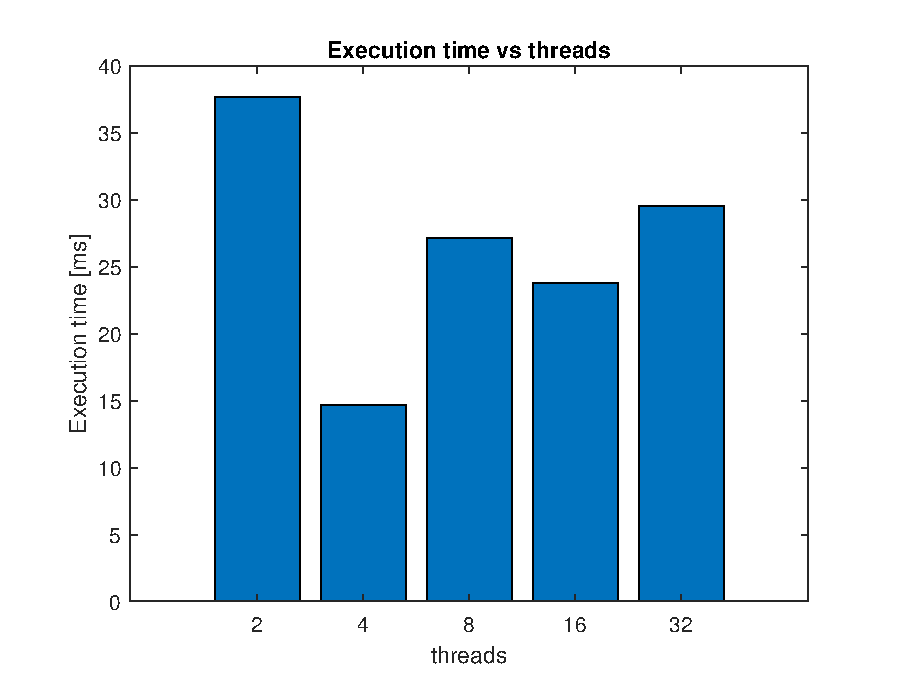
\includegraphics[width = 7cm, height = 7cm]{graph1}

    \caption{Execution time vs Threads}

\end{figure}

\begin{figure}[!h]

    \centering

    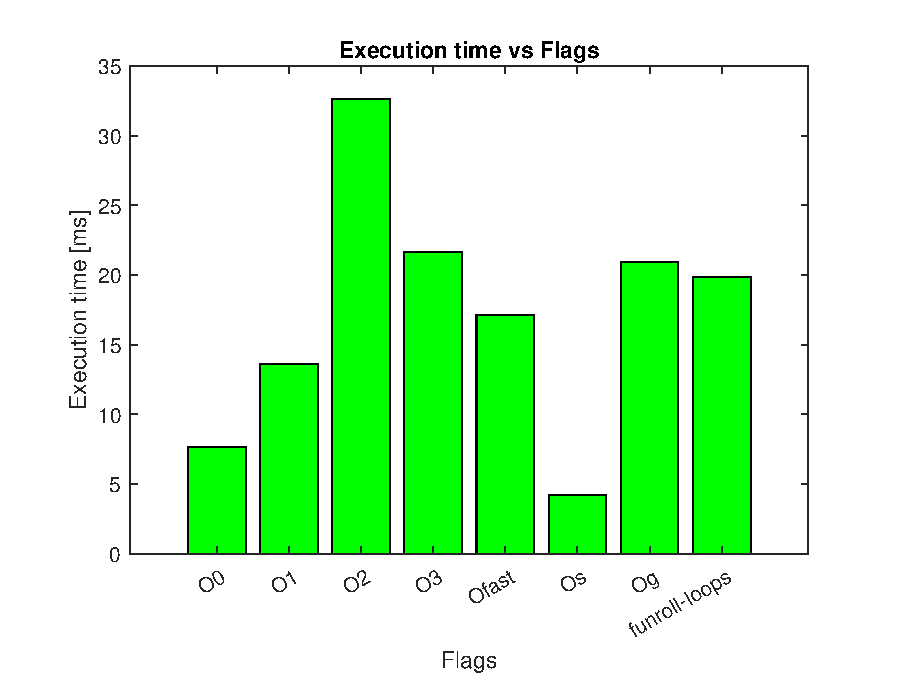
\includegraphics[width = 7cm, height = 7cm]{graph2}

    \caption{Execution time vs Threads}

\end{figure}

13. The execution time for python was 1579.535 ms, and the execution time for C was 46.128 ms. C had a much faster execution time due to python being an interpreted language. The instructions from python are not ran exactly by the CPU, meanwhile C has its code compiled and the instructions are run at a low level much faster.

14.4 No, the code does not run faster as the number of threads increase. The speed increases from 2 threads to 4 threads then it starts to decrease from 8 threads to 32 threads. The raspberry pi has 4 cores, this limits it on much it can improve the speed. When the threads increase beyond 4, this makes the CPU wait for the 4 cores to finish the operation then run the other 4 threads. This dividing and combining of tasks increases the overall time the program takes to run.

17. The flag with the highest speed is -Os, this was unexpected. The expected flag to have the highest speed was -Ofast. This might be due to the pi emulator having small storage. So, when the pi runs the code optimised for storage. 

18. 
Float – 32 bits
Double – 64 bits
fp16 – 16 bits
19. 
The best combination was using 4 threads, -Os, and data size of float. 

\section{Conclusion}

13.
 
tpython = 1579.535 ms and tc = 69.462 ms

The time it took for python code to run is shorter than the time it took the C program to run.

 <comment on this observation>

14.4

Making the pragram run on 2 and 4 threads improved the speed. The started decreased, from thread 8, 16 and 32. Time is spent dividing up and adding up tasks among threads, that is why the speed decreased.

\end{document}